\documentclass[12pt,a4paper,hidelinks]{article}
\usepackage[english,italian]{babel}
\usepackage{float}
\usepackage{amsmath, amssymb, pifont, geometry, tikz, hyperref, newlfont, graphicx, caption, array, multirow, tabularx, svg, pdfpages}
\usepackage{listings}
\renewcommand{\lstlistingname}{Listato}
\usepackage{xcolor}
\usepackage{setspace}
\usepackage{csquotes}
\usepackage{mathrsfs} % https://www.ctan.org/pkg/mathrsfs

\usepackage[
backend=biber,
style=numeric,
sorting=ynt
]{biblatex}

\usepackage{longtable}

\hypersetup{
	bookmarksopen=true,	
	pdfauthor=Riccardo Valtorta
}

\lstdefinestyle{myStyle}{
	language=SQL,
	basicstyle=\small\ttfamily,
	keepspaces=true
}

\lstdefinestyle{myStyle2}{
	language=SQL,
	basicstyle=\small\ttfamily,
	keepspaces=true,
	numbers = left,
	numbersep=1pt
}

\definecolor{codegreen}{rgb}{0,0.6,0}
\definecolor{codegray}{rgb}{0.5,0.5,0.5}
\definecolor{codepurple}{rgb}{0.58,0,0.82}
\definecolor{backcolour}{rgb}{0.95,0.95,0.92}

\lstdefinestyle{myStyle3}{
	language=SQL,
	backgroundcolor=\color{backcolour},   
	commentstyle=\color{codegreen},
	keywordstyle=\color{magenta},
	numberstyle=\tiny\color{codegray},
	stringstyle=\color{codepurple},
	basicstyle=\ttfamily\footnotesize,
	breakatwhitespace=false,         
	breaklines=true,                 
	captionpos=b,                    
	keepspaces=true,                 
	numbers=left,                    
	numbersep=5pt,                  
	showspaces=false,                
	showstringspaces=false,
	showtabs=false,                  
	tabsize=2
}

\lstdefinestyle{py}{
	language=Python,
	backgroundcolor=\color{backcolour},   
	commentstyle=\color{codegreen},
	keywordstyle=\color{magenta},
	numberstyle=\tiny\color{codegray},
	stringstyle=\color{codepurple},
	basicstyle=\ttfamily\footnotesize,
	breakatwhitespace=false,         
	breaklines=true,                 
	captionpos=b,                    
	keepspaces=true,                 
	numbers=left,                    
	numbersep=5pt,                  
	showspaces=false,                
	showstringspaces=false,
	showtabs=false,                  
	tabsize=2
}

\graphicspath{{figures/}}

\begin{document}
	
	\begin{titlepage}
		\begin{center}
			\begin{spacing}{1.5}
				{\Large \textsc{Dipartimento di Ingegneria dell'Informazione}}\\
				{\large \it Corso di Laurea in Ingegneria Informatica}
			\end{spacing}
		\end{center}
		
		\vspace{15mm}
		
		\begin{center}
			\begin{spacing}{1.5}
				{\LARGE \textsc{Optimization Algorithms}}\\
				Lublanis Matteo
			\end{spacing}
		\end{center}
		
		\vspace{35mm}
		
		\noindent
		
		\vspace{25mm}
		
		\begin{center}
			{\large \it Anno Accademico 2025/2026}
		\end{center}
	\end{titlepage}
	
	
	\tableofcontents
	\newpage
	\section{Combinatorial Optimization}
	\paragraph{Problemi di ottimizzazione}
	Un problema di ottimizzazione prevede di trovare una soluzione $x$ tale per cui:
	\begin{equation}
	\begin{aligned}
		& \min \quad & f(x) & \\
		\textrm{s. t} \quad & g_i(x)\ge 0 \quad & i=1\dots m\\
		\quad & h_j(x)=0 \quad & j=1\dots p\\\quad
		& x \ge 0
	\end{aligned}
	\end{equation}
	dove $f$, $g_i$ e $h_j$ sono funzioni generiche in $x\in \mathcal{R}^n_+$.
	
	Possono essere espressi come problemi di \textbf{Programmazione Lineare Mista Intera}:
	\begin{equation}
		\begin{aligned}
			& \min \quad & c^tx+d^ty & \\
			\textrm{s. t} \quad & Ax+By\ge b & \\
			& x,y\ge 0 \quad & \\
			& x intero
		\end{aligned}
	\end{equation}
	dove A, B, c e d hanno solo valori interi. Se $x$ è solo intero, si parla di \textbf{Programmazione Lineare Intera ILP}, se invece è binario di \textbf{Programmazione Binaria Intera BIP}.
	
	Un problema di ottimizzazione combinatoria si differenzia dal modo con il quale va ad esplicitare il problema (la forma con la quale viene descritto), ma essa è ambivalente alla formulazione appena vista. Un problema di ottimizzazione combinatoria (COP) prevede di scegliere un sottoinsieme di elementi di un insieme finito discreto di oggetti tale da essere ottimo, ovvero, seguendo una funzione di ottimizzazione, il suo contenuto dia il risultato migliore.
	\textbf{Def. di min:} sia $N=\{1\dots n\}$ un insieme finito discreto e $\mathcal{F}$ una collezione di sottoinsiemi ammissibili di $\mathcal{N}$. Si associa ad ogni elemento $j\in \mathcal{N}$ un costo $c_j$: definiamo COP il problema di determinare il miglior sottoinsieme di $\mathcal{N}$ tale per cui si ha il costo minimo:
	\begin{equation}
		\min={S\subseteq \mathcal{N}}\{\sum_{j\in S}c_j:S\in \mathcal{F}\}
	\end{equation}
	Un COP può essere formulato come BIP, ILP, MILP. Esempi di COP sono:
	\begin{itemize}
		\item Problema dello zaino \begin{equation}\max_{I\subseteq N}\{\sum_{i\in I}v_i:\sum_{i\in I}w_i\le b\}\end{equation}
		\item Set Partitioning \begin{equation}\min_{T\subseteq N}\{\sum_{j\in T}c_j:\bigcup_{j\in T}S_j=M\}\end{equation}
		\item TSP: Problema commesso viaggiatore ($\pi$ è la permutazione ciclica, il viaggio, N da visitare) \begin{equation}\min_{\pi}\{\sum_{j=1}^nc_{j\pi(j)}:\pi \in T\}\end{equation}
	\end{itemize} 
	
	Consigli da seguire per formulaizone:
	\begin{itemize}
		\item n e m (var e vincoli) piccoli: complessità polinomiale dipende da questi valori;
		\item La formulazione è cruciale, ci si vuole avvicinare il più possibile al convex hull: più la formulazione è stringente meglio è (migliora efficienza nella risoluzione). Si definisce convex hull: \begin{equation}CH(X)\{\sum_{i=1}^k\lambda_ix^i|\sum_{i=1}^k\lambda_i=1, \lambda_i\ge 0, x^i \in X\}\end{equation}
		per $X=\{x^1, x^2,...\}$. è un poliedro con soli estremi interi: se conoscessimo il CH il problema rilassato sarebbe identico al problema originale, ottenendo così un tempo risolutivo molto migliore. Trovare CH è difficile, si fan compromessi. Quando ci si avvicina al CH determina la qualità di una formulazione di un problema ($P_a\subset P_b$ equivale a dire che la prima formulazione è almeno forte quanto quella di B (può superarla)).
	\end{itemize}
	
	Dimostriamo ora che per ottenere il CH (o buona approssimazione) serve un numero esponenziali di vincoli, per farlo introduciamo l'\textbf{albero ricoprente minimo}: un grafo aciclico con $n-1$ lati (edges) e o non contiene cicli (formulazione A) o è connesso (formulazione B, tocca tutti i nodi dell'insieme).
	Formulazione A:
	\begin{equation}
		\begin{aligned}
			\min \sum_{e\in E}c_ex_e\\
			\sum_{e\in E}x_e=n-1\\
			\sum_{e\in E(S)}x_e\le |S|-1, S\subset N, S\neq \emptyset \\
			x_e\in \{0,1\} \quad e\in E
		\end{aligned}
	\end{equation}
	Formulazione B:
		\begin{equation}
		\begin{aligned}
			\min \sum_{e\in E}c_ex_e\\
			\sum_{e\in E}x_e=n-1\\
			\sum_{e\in \delta(S)}x_e\ge 1, S\subset N, S\neq \emptyset \\
			x_e\in \{0,1\} \quad e\in E
		\end{aligned}
	\end{equation}
	Cambia solo un vincolo: \textbf{Subtour Elimination Formulation} VS \textbf{Cutset Formulation}. 
	
	Si dimostra che:
	\begin{itemize}
		\item $P_a\subset P_b$ e esistono esempi per cui l'inclusione è stretta;
		\item $P_b$ può avere punti estremi frazionari.
	\end{itemize}
	Primo punto: per ogni S, E è dato dall'unione di $E(S), \delta (S), E(N\backslash S)$, che è la sommatoria di tutti gli $x_e$ relativi per insieme, per ogni $x$ in $P_A$ vale il SEC e quindi $\sum_{e\in E(S)}x_e\le |S|-1$ e $\sum_{e\in E(S)}x_e\le |N\backslash S|-1$ in quanto vale che la sommatoria di $x_e$ deve essere $n-1$, quindi otteniamo $\sum_{e\in E(S)}x_e\ge 1$ dimostrando il primo punto.\\
	Secondo punto: soluzione costruita ad hoc per dimostrarlo, $P_A$ è il CH.
	
	Per il problema del perfect matching, la formulazione B diventa migliore.
	\newpage
	
	\section{Local Search Methods}
	\subsection{Euristiche}
	L'obiettivo degli algoritmi euristici è quello di trovare buone soluzioni in tempi irrisori rispetto a quelli che sarebbero necessari usando metodi esatti: richiede tempi polinomiali e fa da compromesso. Un'euristica trova un \textbf{limite superiore} per un problema di minimo (inferiore se di massimo), mentre la soluzione del problema rilassato trova un \textbf{limite inferiore} (e viceversa per il max).
	
	Due tipi di euristiche:
	\begin{itemize}
		\item \textbf{Costruttive}: inizio da soluzione vuota e costruisco iterativamente;
		\item \textbf{Distruttive}: inizio da soluzione ammissibile e inizio a smantellarla per trovare miglioramenti fin quando non ho più mosse.
	\end{itemize}
	
	La differenza è importante in quanto le distruttive richiedono, appunto, una soluzione iniziale, la quale non sempre è facile da ottenere.
	
	Un esempio di euristica costruttiva viene riportata per il TSP:
	\begin{enumerate}
		\item Scegli un vertice da quale partire e considera il self-loop come soluzione iniziale S.
		\item Espandi S aggiungendo uno ad uno i rimanenti vertici fino ad ottenere un ciclo hamiltoniano (percorso chiuso che tocca ogni nodo e torna al punto di partenza).
		
		Questa procedura si divide in due fasi:
		\begin{enumerate}
			\item Seleziona vertice k, non incluso in S, secondo un certo \textbf{criterio}: nearest neighbor (nodo più vicino), farthest insertion (nodo più lontano), arbitrary insertion, cheapest insertion (costo minimo di inserimento).
			\item Inserisci il vertice k in S, tra due vertici u e v: solitamente si vuole minimizzare il costo d'inserimento ($d_{i,j}=c_{i,k}+c_{k,j}-c_{i,j}$ e voglio $d_{u,v}\le d_{i,j} \forall (i,j)\in S$).
		\end{enumerate}
	\end{enumerate}
	Gli algoritmi \textbf{greedy} (o ingordi) sono algoritmi che si basano sulla scelta ottimale basata soltanto sulle informazioni che si hanno ad ogni step: gli algoritmi greedy possono essere definiti ciechi da questo punto di vista, però sono spesso molto veloci e trovano soluzioni necessari per altri algoritmi (come le metaeuristiche). Esempio greedy per il problema dello zaino, è quello di ordinare gli item secondo un rapporto profitto/peso e poi prendere i primi della lista: l'algoritmo può funzionare bene, fin quando non troviamo un caso edge (\href{https://cs.stackexchange.com/questions/41381/knapsack-greedy-approximation-worst-case}{esempio}).
	
	Abbiamo poi due modi di verificare la qualità di un algoritmo: sperimentalmente o studiandone il caso peggiore.
	
	Un altro esempio di algoritmo greedy proposto è quello di nearest neighbor per un problema di TSP: inizio da soluzione vuota, scelgo un nodo, ad ogni iterazione includo nella soluzione parziale il nodo più vicino al nodo attuale sul quale mi trovo, se la soluzione parziale include tutti i nodi allora la soluzione è stata trovata altrimenti continuo a inserire. Questo algoritmo ha tempi polinomiali legati al numero di nodi presenti nell'insieme, però nel caso peggiore può dare una soluzione disastrosa. Esempio in questo caso:
	\begin{center}
		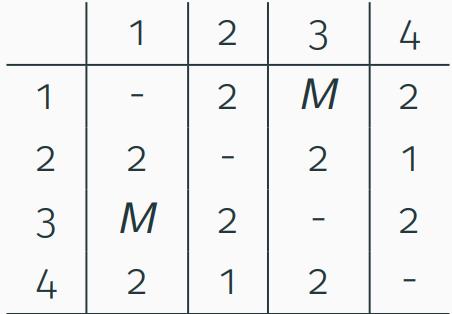
\includegraphics[width=5cm]{tabellacasopeggiore}
	\end{center}
	dove indipendentemente da dove scelgo il nodo iniziale la soluzione dipenderà sempre da M (se $M \le 3$ tutto ok, con $M > 3$ la soluzione che troverà l'algoritmo greedy sarà $\frac{5+M}{8}$ e va all'infinito seguendo M).
	\subsection{Algoritmi di Ricerca Locale}
	\textbf{Neighborhood}: Dato un problema di ottimizzazione $P=(f,S)$ ove $S$ è l'insieme di tutte le soluzioni ammissibili per P e $f:S\rightarrow R$ funzione obiettivo, si definisce neighborhood $N:S\rightarrowtail 2^{|S|}$ tale che $\forall i \in S$ definisca $N(i)\subseteq S$ l'insieme di tutte le soluzioni vicine ad $i$: gli algoritmi di local search cercano di migliorare la soluzione esplorando uno dei neighborhood della soluzione. Su questa definizione si basa tutto il prossimo discorso.
	
	Due algoritmi iterativi migliorativi:
	\begin{itemize}
		\item First Improvement: analizzo vicinati, in ordine random, tengo poi prima soluzione che migliora la f.o; converge a ottimo locale;
		\item Best Improvement: analizzo tutti neighborhood, tengo la soluzione migliore ("steepest descent method" metodo di discesa più ripida), molto più lento ($O(|N(s)|)$ ove $|N(s)|$ è la cardinalità del vicinato).
	\end{itemize}
	
	Gli algoritmi di ricerca locale sono flessibili e applicabili un po' sempre, ma finiscono in ottimi locali purtroppo: per risolvere si usano le metaeuristiche, che implementano metodi per sfuggire agli ottimi locali. Richiedono anche un valutatore di soluzione (f.o), check di ammissibilità per soluzione, funzione di vicinato, tecnica di esplorazione del vicinato efficiente.
	
	\textbf{m-opt}: m archi vengono rimossi nella soluzione del TSP ($G(V,e),c,min)$), poi le strade vengono ricollegate con ancora m archi (2-opt migliore).
	\newpage
	
	\section{Kernel Search}
\end{document}